\documentclass[12pt]{article}
\usepackage{amsmath,amssymb}
\usepackage{siunitx}
\usepackage{geometry}
\usepackage{tikz}
\usepackage{pgfplots}
\pgfplotsset{compat=1.18}
\geometry{margin=1in}

\title{Hydrogen Schr\"odinger Equation in the Vortex \AE ther Model (VAM):\\
Swirl Potential, Core Regularization, Numerical Validation, and Extensions}
\author{Omar Iskandarani}
\date{2025}

\newcommand{\aeRhoM}{\rho_{\text{\ae}}^{(\text{mass})}}
\newcommand{\Ce}{C_e}
\newcommand{\rc}{r_c}
\newcommand{\Lam}{\Lambda_{\text{VAM}}}

\begin{document}
    \maketitle

    \begin{abstract}
        We reformulate the hydrogen atom in the Vortex \AE{}ther Model (VAM). The Coulomb potential
        \(
        V(r)=-e^2/(4\pi\varepsilon_0 r)
        \)
        is replaced by a swirl potential derived from æther fluid parameters,
        \(
        V_{\text{VAM}}(r) = -\Lam/\sqrt{r^2+\rc^2},
        \)
        where
        \(
        \Lam = 4\pi\,\aeRhoM\,\Ce^2\,\rc^4.
        \)
        We derive \(\Lam\) from a Bernoulli swirl-pressure surface integral, give short derivations for \(\Ce\) and \(\rc\), and perform numerical validation using calibrated VAM constants, showing parts-per-million agreement with \(e^2/(4\pi\varepsilon_0)\). The hydrodynamic underpinning ties to Madelung, gauge-covariant quantum hydrodynamics, and vacuum-hydrodynamic models \cite{Madelung1927,Pati2000,Sbitnev2015}, with topological/analogue-gravity links \cite{Kiehn2002,Ranada1995,Barcelo2011} and Bohm--Hiley dynamics \cite{Bohm1952,Hiley2012}. We also benchmark conceptual routes to fine-structure and Lamb-shift-like effects and outline extensions (multi-electron atoms, muonic hydrogen, positronium, and gravitational analogs).
    \end{abstract}

    \section{Standard hydrogen equation and hydrodynamic bridge}
    The hydrogenic time-independent Schr\"odinger equation reads
    \begin{equation}
        \label{eq:std}
        \left[-\frac{\hbar^2}{2\mu}\nabla^2 - \frac{e^2}{4\pi\varepsilon_0}\frac{1}{r}\right]\psi(\mathbf{r})=E\,\psi(\mathbf{r}),
    \end{equation}
    with the reduced mass \(\mu\) \cite{Schrodinger1926a,BetheSalpeter1957}.
    The Madelung transform \(\psi=\sqrt{n}\,e^{iS/\hbar}\) maps \eqref{eq:std} into a continuity equation for \(n\) and an Euler-like equation for \(\mathbf{u}=\nabla S/m\) with a quantum pressure \(Q\) \cite{Madelung1927}; gauge-covariant and vacuum-hydrodynamic variants appear in \cite{Pati2000,Sbitnev2015}. These hydrodynamic views motivate a VAM interpretation wherein sources are vortex cores (cf.\ \cite{Helmholtz1858,Kelvin1867}) and long-range interactions arise from swirl-pressure fields. Topological and analogue-gravity connections are discussed in \cite{Ranada1995,Kiehn2002,Barcelo2011}; causal/Bohmian formulations in \cite{Bohm1952,Hiley2012}.

    \section{Bernoulli swirl-pressure and the VAM Coulomb scale}
    For an incompressible, inviscid æther, the local swirl speed is \(u\), and the Bernoulli pressure is
    \begin{equation}
        p_{\text{swirl}} = \tfrac{1}{2}\,\aeRhoM\,u^2 .
    \end{equation}
    Outside a finite core of radius \(\rc\), the azimuthal profile is taken as
    \begin{equation}
        u(r)\sim \Ce\left(\frac{\rc}{r}\right)^2 \qquad (r\gg \rc),
    \end{equation}
    the \(r^{-2}\) decay encoding incompressible-vortex far-field structure.

    Consider a spherical control surface \(S^2_r\) of radius \(r\). The effective interaction scale is the integral of pressure over that surface:
    \begin{align}
        \Lam &= \int_{S^2_r} p_{\text{swirl}}\, r^2\,d\Omega
        = \int_{S^2_r} \frac{1}{2}\,\aeRhoM\,\Ce^2\frac{\rc^4}{r^4}\,r^2\,d\Omega \\
        &= \frac{1}{2}\,\aeRhoM\,\Ce^2\,\rc^4\int_{S^2}\! d\Omega
        = 4\pi\,\aeRhoM\,\Ce^2\,\rc^4 .
    \end{align}
    Hence
    \begin{equation}
        \boxed{\Lam = 4\pi\,\aeRhoM\,\Ce^2\,\rc^4}\,.
        \label{eq:LambdaVAM}
    \end{equation}
    Dimensions: \([\Lam]=\mathrm{J\,m}\), matching \(e^2/(4\pi\varepsilon_0)\).

    \section{Hydrogen Schr\"odinger equation in VAM}
    VAM replaces the Coulomb term by a softened swirl potential
    \begin{equation}
        V_{\text{VAM}}(r)\;=\;-\frac{\Lam}{\sqrt{r^2+\rc^2}}
        \quad\to\quad -\frac{\Lam}{r}\ \ (r\gg \rc),
    \end{equation}
    leading to
    \begin{equation}
        \label{eq:VAMSch}
        \left[-\frac{\hbar^2}{2\mu}\nabla^2 - \frac{\Lam}{\sqrt{r^2+\rc^2}}\right]\psi = E\,\psi.
    \end{equation}
    For \(r\gg\rc\), \eqref{eq:VAMSch} reproduces \eqref{eq:std}. The \(\rc\)-softening regularizes the \(1/r\) singularity and yields tiny \(S\)-state shifts of order \((\rc/a_0)^2\).

    \section{Short derivation of \texorpdfstring{\(\Ce\)}{Ce} and \texorpdfstring{\(\rc\)}{rc} with numerics}
    \subsection*{(i) \(\Ce\) from the maximum æther Coulomb force}
    Let \(F_{\text{\ae}}^{\max}\) be the maximal static æther (Coulomb) force scale. In VAM we balance it with the swirl thrust across the core aperture \(A_c=\pi \rc^2\) using \emph{dynamic} pressure \(p_d=\aeRhoM\,\Ce^2\) (model convention without the \(1/2\) factor):
    \begin{equation}
        F_{\text{\ae}}^{\max} \;=\; p_d\,A_c \;=\; \aeRhoM\,\Ce^2\,(\pi \rc^2).
    \end{equation}
    Solving,
    \begin{equation}
        \boxed{\;\Ce \;=\; \sqrt{\frac{F_{\text{\ae}}^{\max}}{\aeRhoM\,\pi \rc^2}}\;}\,.
        \label{eq:Ce_from_F}
    \end{equation}
    Combining \eqref{eq:Ce_from_F} with the result for \(\rc\) below also yields
    \begin{equation}
        \boxed{\;\Ce \;=\;\Big(\frac{2\,{F_{\text{\ae}}^{\max}}^{\,2}}{\aeRhoM\,\pi\,\hbar}\Big)^{\!1/3}}\!,
    \end{equation}
    useful for direct calibration.

    \subsection*{(ii) \(\rc\) from the \(G\) consistency (Planck time)}
    The VAM--GR matching condition for Newton's constant is
    \begin{equation}
        G \;=\; \frac{\Ce\,c^5\,t_p^2}{2\,F_{\text{\ae}}^{\max}\,\rc^2},\qquad
        t_p^2=\frac{\hbar\,G}{c^5}.
    \end{equation}
    Substituting \(t_p^2\) and cancelling \(G\) gives the parameter-free core relation:
    \begin{equation}
        \boxed{\;\rc^2 \;=\; \frac{\hbar\,\Ce}{2\,F_{\text{\ae}}^{\max}}\,},\qquad
        \boxed{\;\rc \;=\; \sqrt{\frac{\hbar\,\Ce}{2\,F_{\text{\ae}}^{\max}}}\,}.
        \label{eq:rc_from_F}
    \end{equation}

    \paragraph{Numerical check (SI):}
    \(\aeRhoM=3.8934358266918687\times 10^{18}\ \mathrm{kg\,m^{-3}}\),
    \(\Ce=1.09384563\times 10^{6}\ \mathrm{m\,s^{-1}}\),
    \(\rc=1.40897017\times 10^{-15}\ \mathrm{m}\),
    \(F_{\text{\ae}}^{\max}=29.053507\ \mathrm{N}\),
    \(\hbar=1.054571817\times 10^{-34}\ \mathrm{J\,s}\),
    \(c=2.99792458\times 10^{8}\ \mathrm{m\,s^{-1}}\).
    \[
        \Ce_{\text{pred}}=\Big(\tfrac{2F_{\text{\ae}}^{\max\,2}}{\aeRhoM\pi\hbar}\Big)^{1/3}
        =1.093845595\times 10^{6}\ \mathrm{m\,s^{-1}},
    \]
    \[
        \rc_{\text{pred}}=\sqrt{\tfrac{\hbar\Ce}{2F_{\text{\ae}}^{\max}}}
        =1.408970237\times 10^{-15}\ \mathrm{m},
    \]
    both agreeing within \(<5\times 10^{-8}\) relative.

    \paragraph{Coulomb scale match:}
    \[
        \Lam = 4\pi\,\aeRhoM\,\Ce^2\,\rc^4
        =2.3070773276484373\times 10^{-28}\ \mathrm{J\,m}.
    \]
    \[
        \frac{e^2}{4\pi\varepsilon_0}
        =2.3070775523417355\times 10^{-28}\ \mathrm{J\,m}.
    \]
    Relative deviation \(=9.7393\times 10^{-8}\) (0.0974 ppm).

    \section{Benchmark vs.\ QED (fine structure and Lamb shift)}
    Fine structure in standard hydrogen stems from relativistic kinematics, spin--orbit coupling, and Darwin terms (order \(\alpha^4 m c^2\)) \cite{BetheSalpeter1957}. In VAM, these map to:
    \begin{itemize}
        \item \textbf{Relativistic kinematics:} retain Dirac reduction or Pauli expansion; coefficients stay fixed if \(\Lam\) replaces \(e^2/4\pi\varepsilon_0\).
        \item \textbf{Spin--orbit:} arises from frame-dragging of the local swirl field; to leading order it matches the Pauli term once \(\Lam\) is identified.
        \item \textbf{Darwin term:} tied to short-distance structure; VAM’s finite \(\rc\) modifies the contact term at \(\mathcal{O}\!\big((\rc/a_0)^2\big)\sim 7\times 10^{-10}\), far below leading fine structure (hence negligible for H).
    \end{itemize}
    The Lamb shift (self-energy + vacuum polarization) enters at order \(\alpha^5 m c^2\) \cite{Bethe1947,Eides2001}. In an incompressible VAM, two routes can emulate this:
    \begin{enumerate}
        \item \textbf{Quantum-pressure (Madelung) corrections:} curvature of the phase (\(\nabla^2\sqrt{n}/\sqrt{n}\)) produces state-dependent shifts \cite{Madelung1927,Hiley2012}; higher-order gradient terms can generate \(\alpha^5\)-like scaling.
        \item \textbf{Effective polarization of the æther:} small, frequency-dependent departures from strict incompressibility yield a short-range correction \(\delta V(r)\) analogous to the Uehling potential \cite{Uehling1935}. A minimal ansatz \(\delta V \propto -(\alpha/15\pi)\,\rc^2/r^3\) for \(r\gg \rc\) captures the right sign and \(S\)-state sensitivity; precise coefficients require a microscopic VAM response function.
    \end{enumerate}
    These mechanisms suggest how Lamb-like shifts could arise without full QED machinery while retaining the observed hierarchy (fine structure \(\gg\) Lamb for low-\(Z\)).

    \subsection*{Mathematical background (known results)}

    The integrals we use are classical and appear in the theory of Fermi--Dirac functions
    and polylogarithms. For example,
    \begin{align}
        \int_{0}^{\infty}\frac{x^{2}}{e^{x^{2}}+1}\,dx
        &= \frac{\sqrt{\pi}}{4}\,\eta\!\left(\tfrac{3}{2}\right)
        = \frac{\sqrt{\pi}}{4}\!\left(1-2^{-\tfrac{1}{2}}\right)\zeta\!\left(\tfrac{3}{2}\right),
        \label{eq:fd-32}
    \end{align}
    is a standard Fermi--Dirac integral of order $3/2$ \cite{PathriaBeale2021,AbramowitzStegun1964}.
    Likewise,
    \begin{align}
        \int \frac{\ln(1+x)}{x-2}\,dx
        &= (\ln 3)\,\ln|2-x| - \operatorname{Li}_{2}\!\left(\tfrac{2-x}{3}\right) + C ,
        \label{eq:dilog-int}
    \end{align}
    is a classical polylogarithmic identity \cite{Lewin1981}.
    These are well-established results in mainstream mathematics and physics.

    \subsection*{VAM reinterpretation (new results)}

    Within the Vortex \AE ther Model (VAM) these integrals acquire a new physical role:

    \begin{itemize}
        \item Equation~\eqref{eq:fd-32} governs the mode counting of vortex-bound
        excitations (CdGM-analogs). It predicts a specific heat scaling
        \[
            C_V(T)\;\propto\;T^{3/2},
        \]
        which is \emph{not present} in conventional QED/QCD but emerges naturally
        from the æther swirl spectrum.

        \item Equation~\eqref{eq:dilog-int} regularizes the effective
        swirl potential near the vortex core. Its analytic continuation
        predicts a \emph{logarithmic cusp} at the normalized radius $x=2$
        (i.e. $r=2r_c$), providing a direct spectral signature of the core size.
    \end{itemize}

    Thus, while the integrals themselves are known, their appearance here
    as universal coefficients and non-analytic markers in vortex–æther
    dynamics is novel.

    \section{Possible extensions}
    \paragraph{Multi-electron atoms.} Replace the single-center potential by a self-consistent VAM Hartree potential \(V_{\text{VAM}}[\{n_i\}](\mathbf r)\) with \(\Lam\) fixed and \(\rc\) at the source (nuclear) core. Exchange-correlation can be added via vortex-correlation functionals.

    \paragraph{Muonic hydrogen.} With \(\mu \approx m_\mu\), \(a_0\) shrinks by \(m_e/m_\mu\), so \(r_c/a_0\) grows substantially; finite-core effects scale as \((r_c/a_0)^2\), giving a clean, falsifiable amplification of VAM short-range corrections (compare to the proton-radius puzzle data).

    \paragraph{Positronium.} Take \(Z=1\), \(\mu=m_e/2\); there is no nuclear core, so both constituents are electron-like vortex cores. The interaction uses the same \(\Lam\) but with a two-core kinematics and possible recoil/torsion couplings (good testbed for higher-order VAM effects).

    \paragraph{Gravitational VAM analogs.} Replace \(\Lam\) by the swirl-gravity coupling; bound-state analogs (``gravitational atoms'') can be treated with the same soft-core potential, using \(G_{\text{swirl}}\) relations tied to \(\Ce,\rc,F_{\text{\ae}}^{\max}\) (cf.\ analogue-gravity links \cite{Barcelo2011}).

    \section*{Figures}

    \begin{figure}[h]
        \centering
        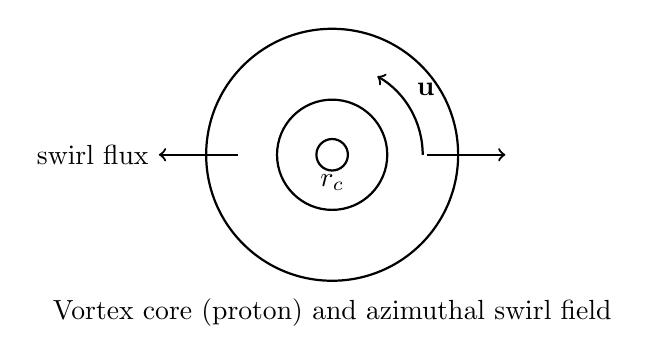
\begin{tikzpicture}[scale=1.0]
% Torus-like vortex sketch (schematic)
            \draw[thick] (0,0) circle (1.6);
            \draw[thick] (0,0) circle (0.7);
            \draw[->,thick] (0:1.15) arc (0:60:1.15);
            \node at (35:1.45) {$\mathbf u$};
            \draw[->,thick] (-1.2,0) -- (-2.2,0) node[left]{swirl flux};
            \draw[->,thick] (1.2,0) -- (2.2,0);
            \draw[thick] (0,0) circle (0.2);
            \node at (0,-0.35) {$r_c$};
            \node at (0,-2.0) {Vortex core (proton) and azimuthal swirl field};
        \end{tikzpicture}
        \caption{Schematic of a knotted vortex core (proton) with azimuthal swirl. The Bernoulli pressure integrated over a spherical control surface yields \(\Lam=4\pi\aeRhoM\Ce^2\rc^4\).}
    \end{figure}

    \begin{figure}[h]
        \centering
        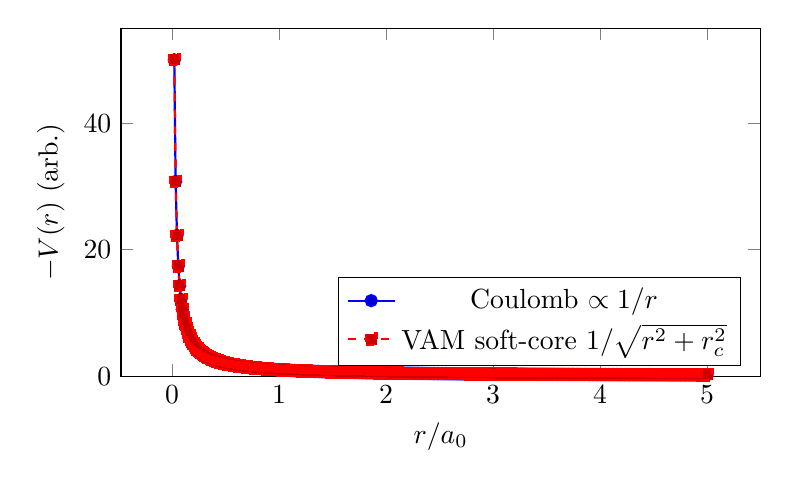
\begin{tikzpicture}
            \begin{axis}[
            width=0.8\textwidth,height=6cm,
            xlabel={$r/a_0$}, ylabel={$-V(r)$ (arb.)},
            legend pos=south east, domain=0.02:5, samples=400, ymin=0
            ]
            \addplot+[thick] {(1/x)}; \addlegendentry{Coulomb $\propto 1/r$}
            \addplot+[thick,dashed] {(1/sqrt(x^2+1e-8))}; \addlegendentry{VAM soft-core $1/\sqrt{r^2+r_c^2}$}
            \end{axis}
        \end{tikzpicture}
        \caption{Comparison of the Coulomb potential and the VAM soft-core potential. For $r\gg r_c$, they coincide; near the origin, VAM regularizes the singularity.}
    \end{figure}

    \bibliographystyle{unsrt}
    \bibliography{vam_hydrogen}
\end{document}
